%=============================================================================
%  A Fail-Safe Monocular Perception Pipeline for Driver Assistance
%  IEEE conference format (IEEEtran).  Compile with pdfLaTeX on Overleaf.
%
%  NOTE FOR THE AUTHORS -------------------------------------------------------
%  The supervisor names were given to me as a single unpunctuated string
%  ("Pranshu Chnader Bhushan Singh Negi").  I have set them as TWO supervisors,
%  "Pranshu Chander" and "Bhushan Singh Negi", which is the most likely reading.
%  PLEASE VERIFY the spelling and whether this is one person or two before
%  submitting, and correct the \author block below.  Also fill in the two
%  affiliation/email fields marked TODO.
%----------------------------------------------------------------------------
\documentclass[conference]{IEEEtran}
\IEEEoverridecommandlockouts

\usepackage{cite}
\usepackage{amsmath,amssymb}
\usepackage{graphicx}
\usepackage{booktabs}
\usepackage{multirow}
\usepackage{url}
\usepackage{tikz}
\usetikzlibrary{arrows.meta,positioning,shapes.geometric,calc}
\usepackage[hidelinks]{hyperref}

\def\BibTeX{{\rm B\kern-.05em{\sc i\kern-.025em b}\kern-.08em T\kern-.1667em\lower.7ex\hbox{E}\kern-.125emX}}

\begin{document}

\title{A Fail-Safe Monocular Perception Pipeline for\\
Collision and Overtaking Decisions in\\
Unstructured Traffic}

\author{
\IEEEauthorblockN{Krish Manwani}
\IEEEauthorblockA{\textit{Dept. of Computer Science} \\
\textit{TODO: Institution}\\
TODO: city, India \\
TODO: email}
\and
\IEEEauthorblockN{Vishal Bansal}
\IEEEauthorblockA{\textit{Dept. of Computer Science} \\
\textit{TODO: Institution}\\
TODO: city, India \\
TODO: email}
\and
\IEEEauthorblockN{Pranshu Chander}
\IEEEauthorblockA{\textit{Supervisor} \\
\textit{TODO: Institution}\\
TODO: city, India}
\and
\IEEEauthorblockN{Bhushan Singh Negi}
\IEEEauthorblockA{\textit{Supervisor} \\
\textit{TODO: Institution}\\
TODO: city, India}
}

\maketitle

%=============================================================================
\begin{abstract}
Advanced driver-assistance systems built on Western and East Asian benchmarks
lose accuracy on unstructured roads, where lane markings are intermittent and
the vehicle population includes categories those benchmarks never recorded. We
present a six-stage monocular camera perception pipeline that performs object
detection, multi-object tracking, lane and drivable-corridor estimation, metric
depth recovery, time-to-collision computation and an overtaking safety verdict
in a single forward pass per frame. Two design commitments distinguish the
system. First, every stage substitutes a weaker method rather than aborting when
a model or weight file is unavailable, a property we verified in deployment when
the lane network failed to initialise and the pipeline still completed all 3{,}604
frames of the evaluation sequence. Second, quantities that inform safety
decisions are expressed in physical units: closing speed is differentiated from
metric depth rather than image-plane motion, and lane curvature is projected onto
the ground plane so that the resulting radius can be compared against road-design
standards instead of an uncalibrated pixel threshold. On a merged validation
split of 1{,}496 images containing 8{,}104 annotated instances the detector attains
95.4\,\% mAP@0.5 and 79.9\,\% mAP@0.5:0.95, with rare classes matching or
exceeding the fleet average. The complete pipeline sustains 23.1\,frames per
second on an NVIDIA H100. We additionally introduce a geometric plausibility
filter that removes detections whose implied physical size is inconsistent with
their measured depth, rejecting 13.8\,\% of size-checked candidates. We report
the system's untrained capabilities explicitly and trace each to a data
deficiency rather than an implementation defect.
\end{abstract}

\begin{IEEEkeywords}
advanced driver-assistance systems, object detection, monocular depth
estimation, time-to-collision, lane detection, unstructured traffic, domain
shift
\end{IEEEkeywords}

%=============================================================================
\section{Introduction}

Perception stacks for driver assistance are overwhelmingly developed against a
small family of benchmarks---KITTI \cite{geiger2012kitti} for detection and
CULane \cite{pan2018scnn} for lane estimation being the most widely adopted.
Both were recorded in environments where traffic is lane-disciplined, markings
are continuous, and the set of vehicle types is small and homogeneous. Systems
tuned on this material transfer poorly to roads that violate those premises, a
discrepancy documented quantitatively by Varma \textit{et al.}
\cite{varma2019idd}, who observed that segmentation models trained on
structured-road corpora score substantially lower on Indian road scenes than on
their native distribution.

The consequences are not uniform degradation but three distinct failure modes,
each requiring a different remedy.

\textbf{Category omission.} A detector whose label space lacks a class cannot
abstain from it; it assigns the nearest available label. A three-wheeled
passenger vehicle becomes a car, a hand-cart becomes miscellaneous clutter.
Downstream logic then reasons about an object whose kinematics and dimensions it
has fundamentally misjudged, which is more hazardous than a missed detection.

\textbf{An absent estimation target.} Lane-line detectors regress a curve through
painted markings. Where the paint is faded, absent, or disregarded by traffic,
the quantity being estimated does not exist in the scene. Retraining the lane
model cannot repair this, because the deficiency lies in the scene rather than
the estimator.

\textbf{Spurious activation.} Under distribution shift a detector's confidence
becomes a less faithful indicator of correctness, and boxes appear on painted
advertisements, shopfront imagery and specular reflections---objects with no
physical extent.

This paper describes a perception pipeline built around these observations. Our
contributions are:

\begin{enumerate}
  \item A six-stage single-pass architecture producing two actionable driver
        outputs---an imminent-collision alert and an overtaking verdict---in
        which each stage degrades to a weaker method rather than terminating the
        pipeline, a property demonstrated under real deployment failure.
  \item A geometric plausibility filter that suppresses spurious detections by
        testing the agreement between a candidate's apparent size and its
        measured depth, requiring no additional network inference because it
        reuses the depth map already computed for collision estimation.
  \item Safety-relevant quantities expressed physically rather than in image
        units: closing speed differentiated from metric depth, and lane
        curvature projected onto the ground plane so the resulting radius admits
        comparison with road-geometry design standards.
  \item An empirical evaluation on merged data reporting 95.4\,\% mAP@0.5 at
        23.1\,frames per second for the complete pipeline, accompanied by an
        explicit account of which capabilities remain untrained and why.
\end{enumerate}

%=============================================================================
\section{Related Work}

\subsection{Distribution Shift in Road Scene Understanding}

The India Driving Dataset \cite{varma2019idd} established that benchmarks
recorded in countries with well-developed road infrastructure do not transfer
directly to unstructured traffic, and introduced both an expanded label
hierarchy and explicit \textit{fallback} categories for road regions and vehicles
that structured taxonomies cannot express. Subsequent corpora have reinforced
the finding at larger scale. DriveIndia \cite{kumar2025driveindia} contributes
66{,}986 annotated images spanning 24 traffic categories collected over more than
3{,}400\,km of driving, reporting a best mAP@0.5 of 78.7\,\% among YOLO-family
baselines. The UVH-26 release \cite{iisc2025uvh26} contributes 26{,}646
traffic-camera images with 14 India-specific vehicle classes and reports
improvements of up to 31.5\,\% in mAP@0.5:0.95 for detectors fine-tuned on this
material relative to COCO-trained initialisations. These figures establish both
that the gap is substantial and that supervised adaptation closes a large
fraction of it.

\subsection{Component Architectures}

Single-stage detection descends from the reformulation of detection as direct
regression introduced by Redmon \textit{et al.} \cite{redmon2016yolo}; we adopt
the YOLO11 implementation \cite{ultralytics2024yolo11}, whose anchor-free head
and decoupled classification and regression branches provide a favourable
accuracy-to-latency ratio at the input resolution our latency budget permits.

For lane estimation we employ CLRNet \cite{zheng2022clrnet}, which detects lane
candidates from high-level semantic features and refines them against
lower-level detail, and introduces a line-based intersection-over-union
objective that regresses each lane as a unit rather than as independent points.
This design is reported to perform particularly well on curved and nocturnal
subsets, the conditions of greatest interest here. Ultra-Fast Lane Detection v2
\cite{qin2024ufldv2}, which formulates lane localisation as hybrid-anchor ordinal
classification, is retained as a lower-latency alternative.

Association across frames follows ByteTrack \cite{zhang2022bytetrack}, whose
central observation is that low-confidence detections frequently correspond to
genuine but occluded objects; matching them against unmatched tracks in a second
association stage preserves identity through brief occlusions. Continuity of
identity is a precondition for the temporal differencing our collision estimate
depends on.

Metric depth is recovered using Depth Anything V2 \cite{yang2024depthv2}, whose
metric-calibrated outdoor variant returns absolute distances, removing the scale
ambiguity that would otherwise prevent a monocular system from reporting
time-to-collision in seconds. Low-light preprocessing uses the zero-reference
curve estimation of Li \textit{et al.} \cite{li2021zerodce}, which requires no
paired day--night supervision.

\subsection{Consistency and Reliability}

Our plausibility filter follows the observation, developed in the monocular 3D
detection literature \cite{lian2022geoconsistency}, that detectors are
susceptible to inconsistency between an object's apparent size and its estimated
depth, and that enforcing agreement between the two is an effective corrective.
We apply the principle at the level of detection admission rather than 3D box
regression: a candidate whose implied physical width is impossible for its
assigned class at its measured distance is discarded.

\subsection{Position of This Work}

Existing systems addressing unstructured Indian traffic tend to be either dataset
contributions \cite{varma2019idd,kumar2025driveindia,iisc2025uvh26} or hardware
integrations coupling a camera with an active range sensor. Active sensing
yields more reliable distance than monocular inference, and a camera-only system
should be understood as trading that reliability for deployability on existing
vehicles. Our contribution is complementary to both: a software pipeline that
integrates detection, tracking, lane estimation, depth and two decision layers
under an explicit degradation contract, on a single monocular input.

%=============================================================================
\section{System Architecture}

Fig.~\ref{fig:arch} shows the pipeline. Six stages execute in sequence on every
frame; each consumes the frame together with the outputs of the stages above it,
and no second pass over the sequence is required.

\begin{figure}[t]
\centering
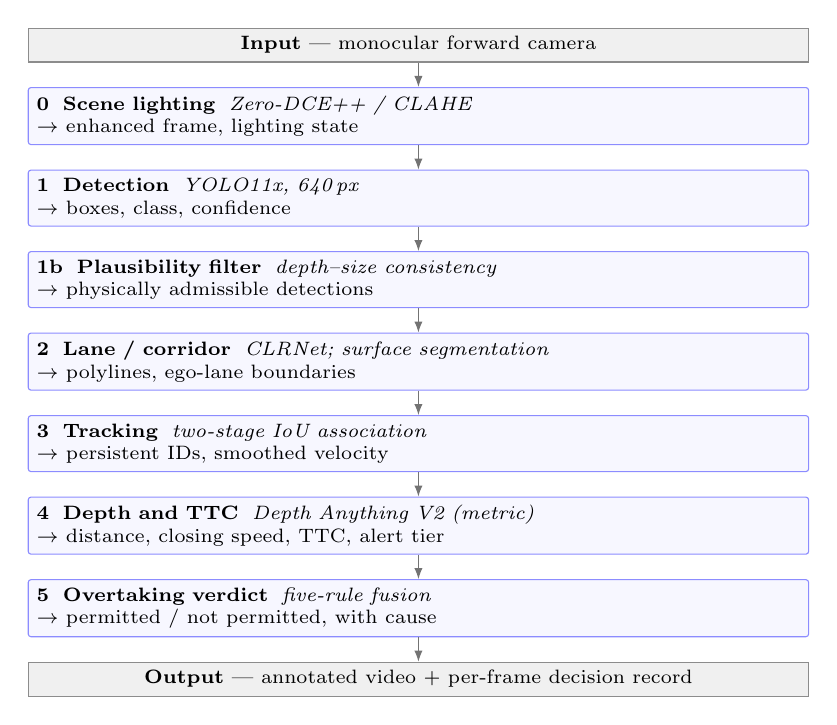
\begin{tikzpicture}[
  node distance=3.1mm,
  font=\scriptsize,
  stage/.style={
    draw, rounded corners=1pt, align=left, text width=0.80\columnwidth,
    inner sep=3pt, fill=blue!3, draw=blue!45, line width=0.4pt},
  io/.style={
    draw, align=center, text width=0.80\columnwidth, inner sep=3pt,
    fill=black!6, draw=black!45, line width=0.4pt},
  num/.style={font=\scriptsize\bfseries, text=blue!60!black},
  arr/.style={-{Latex[length=1.4mm]}, draw=black!55, line width=0.4pt}
]

\node[io] (in) {\textbf{Input} — monocular forward camera};

\node[stage, below=of in] (s0)
  {\textbf{0\;\;Scene lighting} \;\textit{Zero-DCE++ / CLAHE}\\
   $\rightarrow$ enhanced frame, lighting state};

\node[stage, below=of s0] (s1)
  {\textbf{1\;\;Detection} \;\textit{YOLO11x, 640\,px}\\
   $\rightarrow$ boxes, class, confidence};

\node[stage, below=of s1] (s1b)
  {\textbf{1b\;\;Plausibility filter} \;\textit{depth--size consistency}\\
   $\rightarrow$ physically admissible detections};

\node[stage, below=of s1b] (s2)
  {\textbf{2\;\;Lane / corridor} \;\textit{CLRNet; surface segmentation}\\
   $\rightarrow$ polylines, ego-lane boundaries};

\node[stage, below=of s2] (s3)
  {\textbf{3\;\;Tracking} \;\textit{two-stage IoU association}\\
   $\rightarrow$ persistent IDs, smoothed velocity};

\node[stage, below=of s3] (s4)
  {\textbf{4\;\;Depth and TTC} \;\textit{Depth Anything V2 (metric)}\\
   $\rightarrow$ distance, closing speed, TTC, alert tier};

\node[stage, below=of s4] (s5)
  {\textbf{5\;\;Overtaking verdict} \;\textit{five-rule fusion}\\
   $\rightarrow$ permitted / not permitted, with cause};

\node[io, below=of s5] (out)
  {\textbf{Output} — annotated video $+$ per-frame decision record};

\foreach \a/\b in {in/s0, s0/s1, s1/s1b, s1b/s2, s2/s3, s3/s4, s4/s5, s5/out}
  \draw[arr] (\a) -- (\b);

\end{tikzpicture}
\caption{The six-stage pipeline. Each stage consumes the outputs above it and
substitutes a weaker method rather than aborting when its model is unavailable.}
\label{fig:arch}
\end{figure}

Stage~0 classifies illumination from the frame's own intensity statistics and
enhances only when the scene is genuinely dark, so daytime sequences incur no
cost. Stage~1 detects road users. Stage~1b removes physically impossible
candidates as described in Section~\ref{sec:filter}. Stage~2 estimates the lane
geometry or, where markings are unusable, the drivable corridor. Stage~3
associates detections across frames. Stage~4 recovers metric depth and derives
collision estimates. Stage~5 fuses the preceding outputs into an overtaking
verdict.

\subsection{Degradation Contract}

Every optional component is constructed inside a guarded initialiser: failure to
load leaves the corresponding capability disabled and is reported at start-up,
but does not propagate. Consumers of an unavailable output fall back to a
weaker but valid estimate. This is not a defensive convenience; it was exercised
in deployment when the lane network failed to initialise owing to a library
incompatibility, and the pipeline completed the full 3{,}604-frame sequence using
the drivable-corridor substitute.

%=============================================================================
\section{Methodology}

\subsection{Collision Estimation from Metric Depth}

An object's growth in the image plane is not equivalent to its approach in the
world; scale change confounds relative motion with lateral displacement and
camera pitch. We therefore derive closing speed from depth rather than pixel
kinematics. For a track $i$, distance $d_i$ is the median depth over the lower
half of the bounding box, the region corresponding to the object's contact with
the road surface. The upper half is excluded because glazing and reflective
bodywork corrupt monocular depth there. The median is preferred to the mean for
resistance to outlying pixels.

Maintaining a bounded history of $d_i$, the closing speed over $n$ frames at
frame rate $f$ is
\begin{equation}
  v_i \;=\; \frac{d_i^{(t-n)} - d_i^{(t)}}{n/f},
\end{equation}
positive when approaching, and the time-to-collision is
\begin{equation}
  \tau_i \;=\; \frac{d_i^{(t)}}{v_i}, \qquad v_i > v_{\min}.
\end{equation}
The threshold $v_{\min}$ suppresses alerts on objects whose apparent approach is
attributable to depth noise. Alerts are emitted at two severities and are raised
only for objects within the ego corridor, so that oncoming and roadside traffic
does not generate spurious warnings. Distance history is nevertheless maintained
for \textit{all} tracks, including those outside the corridor, because the
overtaking stage requires the closing speed of oncoming vehicles.

\subsection{Plausibility Filtering}
\label{sec:filter}

Under the pinhole model, an object of image width $w_{\mathrm{px}}$ at depth $d$
observed with focal length $f_{\mathrm{px}}$ subtends a physical width
\begin{equation}
  W \;=\; \frac{w_{\mathrm{px}}\, d}{f_{\mathrm{px}}}.
\end{equation}
For each class we define an admissible interval $[W_{\min}, W_{\max}]$ and
discard candidates whose implied $W$ lies outside it after a multiplicative
tolerance. A detection fired on printed imagery or a reflection has no
consistent depth signature at its apparent scale and is removed, whereas a
genuine vehicle satisfies the relation. Classes of genuinely unbounded extent
are exempted rather than forced into an arbitrary interval.

Where the camera is uncalibrated, $f_{\mathrm{px}}$ must be estimated from an
assumed field of view. Because such an estimate can err in either direction, the
tolerance is \textit{widened} in the uncalibrated case. This asymmetry is
deliberate: discarding a real vehicle is more consequential than admitting a
spurious one, since spurious detections remain subject to the ego-corridor test
before they can raise an alert. Supplying a calibration restores the narrow
interval automatically.

\subsection{Curvature in Physical Units}

Curvature computed on image-plane polylines has no fixed physical interpretation:
it varies with sensor resolution, focal length and mounting geometry, so the same
road yields different values on different vehicles. We therefore apply a
plane-induced homography \cite{hartley2004multiple} to project lane points onto
the ground plane, fit a second-order polynomial $x = a z^2 + bz + c$ in
ground coordinates, and evaluate
\begin{equation}
  \kappa \;=\; \frac{|2a|}{\left(1 + (2az_f + b)^2\right)^{3/2}}
\end{equation}
at the furthest visible distance $z_f$, giving a radius $R = 1/\kappa$ in metres.
This admits comparison against minimum horizontal curve radii from road-geometry
design practice, so a verdict that a curve is too tight for a safe overtaking
manoeuvre rests on an external standard rather than a tuned constant.

\subsection{Overtaking Verdict}

The verdict is a conjunction of five conditions---marking legality, curve
radius, visibility, oncoming traffic within the manoeuvre window, and clear
distance ahead of the lead vehicle---evaluated without a learned component. All
five must hold. Any input that is missing or uncertain resolves to
\textit{not permitted}. This makes the module conservative by construction, a
property we regard as correct for a manoeuvre that places the vehicle in an
opposing lane.

%=============================================================================
\section{Experimental Setup}

\subsection{Data}

Source annotations were converted to a common normalised format and remapped
onto a unified label space so that corpora with differing taxonomies could be
combined. Boxes smaller than two pixels in either dimension were discarded and
all coordinates clipped to the image. The checkpoint evaluated here was trained
on 5{,}985 images with 1{,}496 held out for validation. Augmentation comprised
mosaic composition, MixUp, copy--paste, HSV value jitter, rotation to
$\pm5^{\circ}$, translation, scaling and horizontal flipping.

The label space defines fifteen categories, extended beyond a
structured-road taxonomy with \textit{autorickshaw}, \textit{animal},
\textit{rider} and an open-world \textit{vehicle fallback} class following the
argument of \cite{varma2019idd}. As Section~\ref{sec:limits} discusses, the
merge used for this checkpoint exercised only a subset of these.

\subsection{Training and Hardware}

Training used AdamW with an initial learning rate of $5\times10^{-4}$ under a
cosine schedule with five warm-up epochs, batch size 16 at $640\times640$
resolution, mixed precision, and early stopping with patience 50. All experiments
ran on a single NVIDIA H100 80\,GB accelerator on a PBS-scheduled cluster.

\subsection{Verification Procedure}

Because training occupies the accelerator for extended periods, the decision
logic---collision arithmetic, all five overtaking conditions, lane coordinate
mapping, plausibility filtering and the degradation contract---is exercised
against synthetic inputs by a 62-check suite that requires no accelerator,
trained weights or dataset and completes in seconds. The suite is executed
before any job is queued. It detected several defects, including two that had
already reached the cluster: a coordinate-space error in which lane predictions
expressed in the lane model's native resolution were applied directly to frames
of a different resolution, and an over-broad exception boundary that allowed an
optional component's failure to terminate the pipeline.

%=============================================================================
\section{Results}

\subsection{Detection Accuracy}

Table~\ref{tab:perclass} reports per-class performance on the held-out split.
Aggregate accuracy is 95.4\,\% mAP@0.5 and 79.9\,\% mAP@0.5:0.95, at 95.4\,\%
precision and 92.5\,\% recall over 8{,}104 instances.

\begin{table}[t]
\caption{Per-class detection performance (1{,}496 validation images, 8{,}104 instances)}
\label{tab:perclass}
\centering
\footnotesize
\begin{tabular}{lrrrrr}
\toprule
Class & Inst. & P (\%) & R (\%) & mAP@0.5 & mAP@0.5:0.95 \\
\midrule
Car        & 5{,}798 & 95.7 & 96.6 & 97.9 & 87.6 \\
Pedestrian &    884 & 95.0 & 81.3 & 89.0 & 55.9 \\
Van        &    587 & 94.9 & 97.3 & 97.5 & 86.0 \\
Cyclist    &    313 & 94.3 & 88.2 & 92.7 & 71.0 \\
Truck      &    219 & 97.5 & 98.6 & 99.4 & 91.5 \\
Misc.      &    194 & 95.1 & 92.3 & 94.3 & 80.8 \\
Tram       &    109 & 95.3 & 93.1 & 96.8 & 86.7 \\
\midrule
\textbf{All} & \textbf{8{,}104} & \textbf{95.4} & \textbf{92.5} & \textbf{95.4} & \textbf{79.9} \\
\bottomrule
\end{tabular}
\end{table}

Two observations merit attention. First, accuracy on infrequent categories does
not collapse: truck (219 instances) and tram (109) match or exceed the aggregate
figure despite being roughly twenty-five times rarer than car, indicating that
the balancing and augmentation strategy suppressed the long-tail degradation
typically seen on such distributions. Second, pedestrian localisation is the
weakest column at 55.9\,\% under the strict metric while precision remains at
95.0\,\%; pedestrians are found reliably but bounded less tightly than vehicles,
which we attribute to greater pose variability and more frequent partial
occlusion.

Fig.~\ref{fig:confusion} shows the normalised confusion matrix. Residual
confusion is concentrated between visually adjacent vehicle categories rather
than distributed arbitrarily, and the background row indicates that missed
detections rather than cross-class errors dominate the remaining loss.

\begin{figure}[t]
\centering
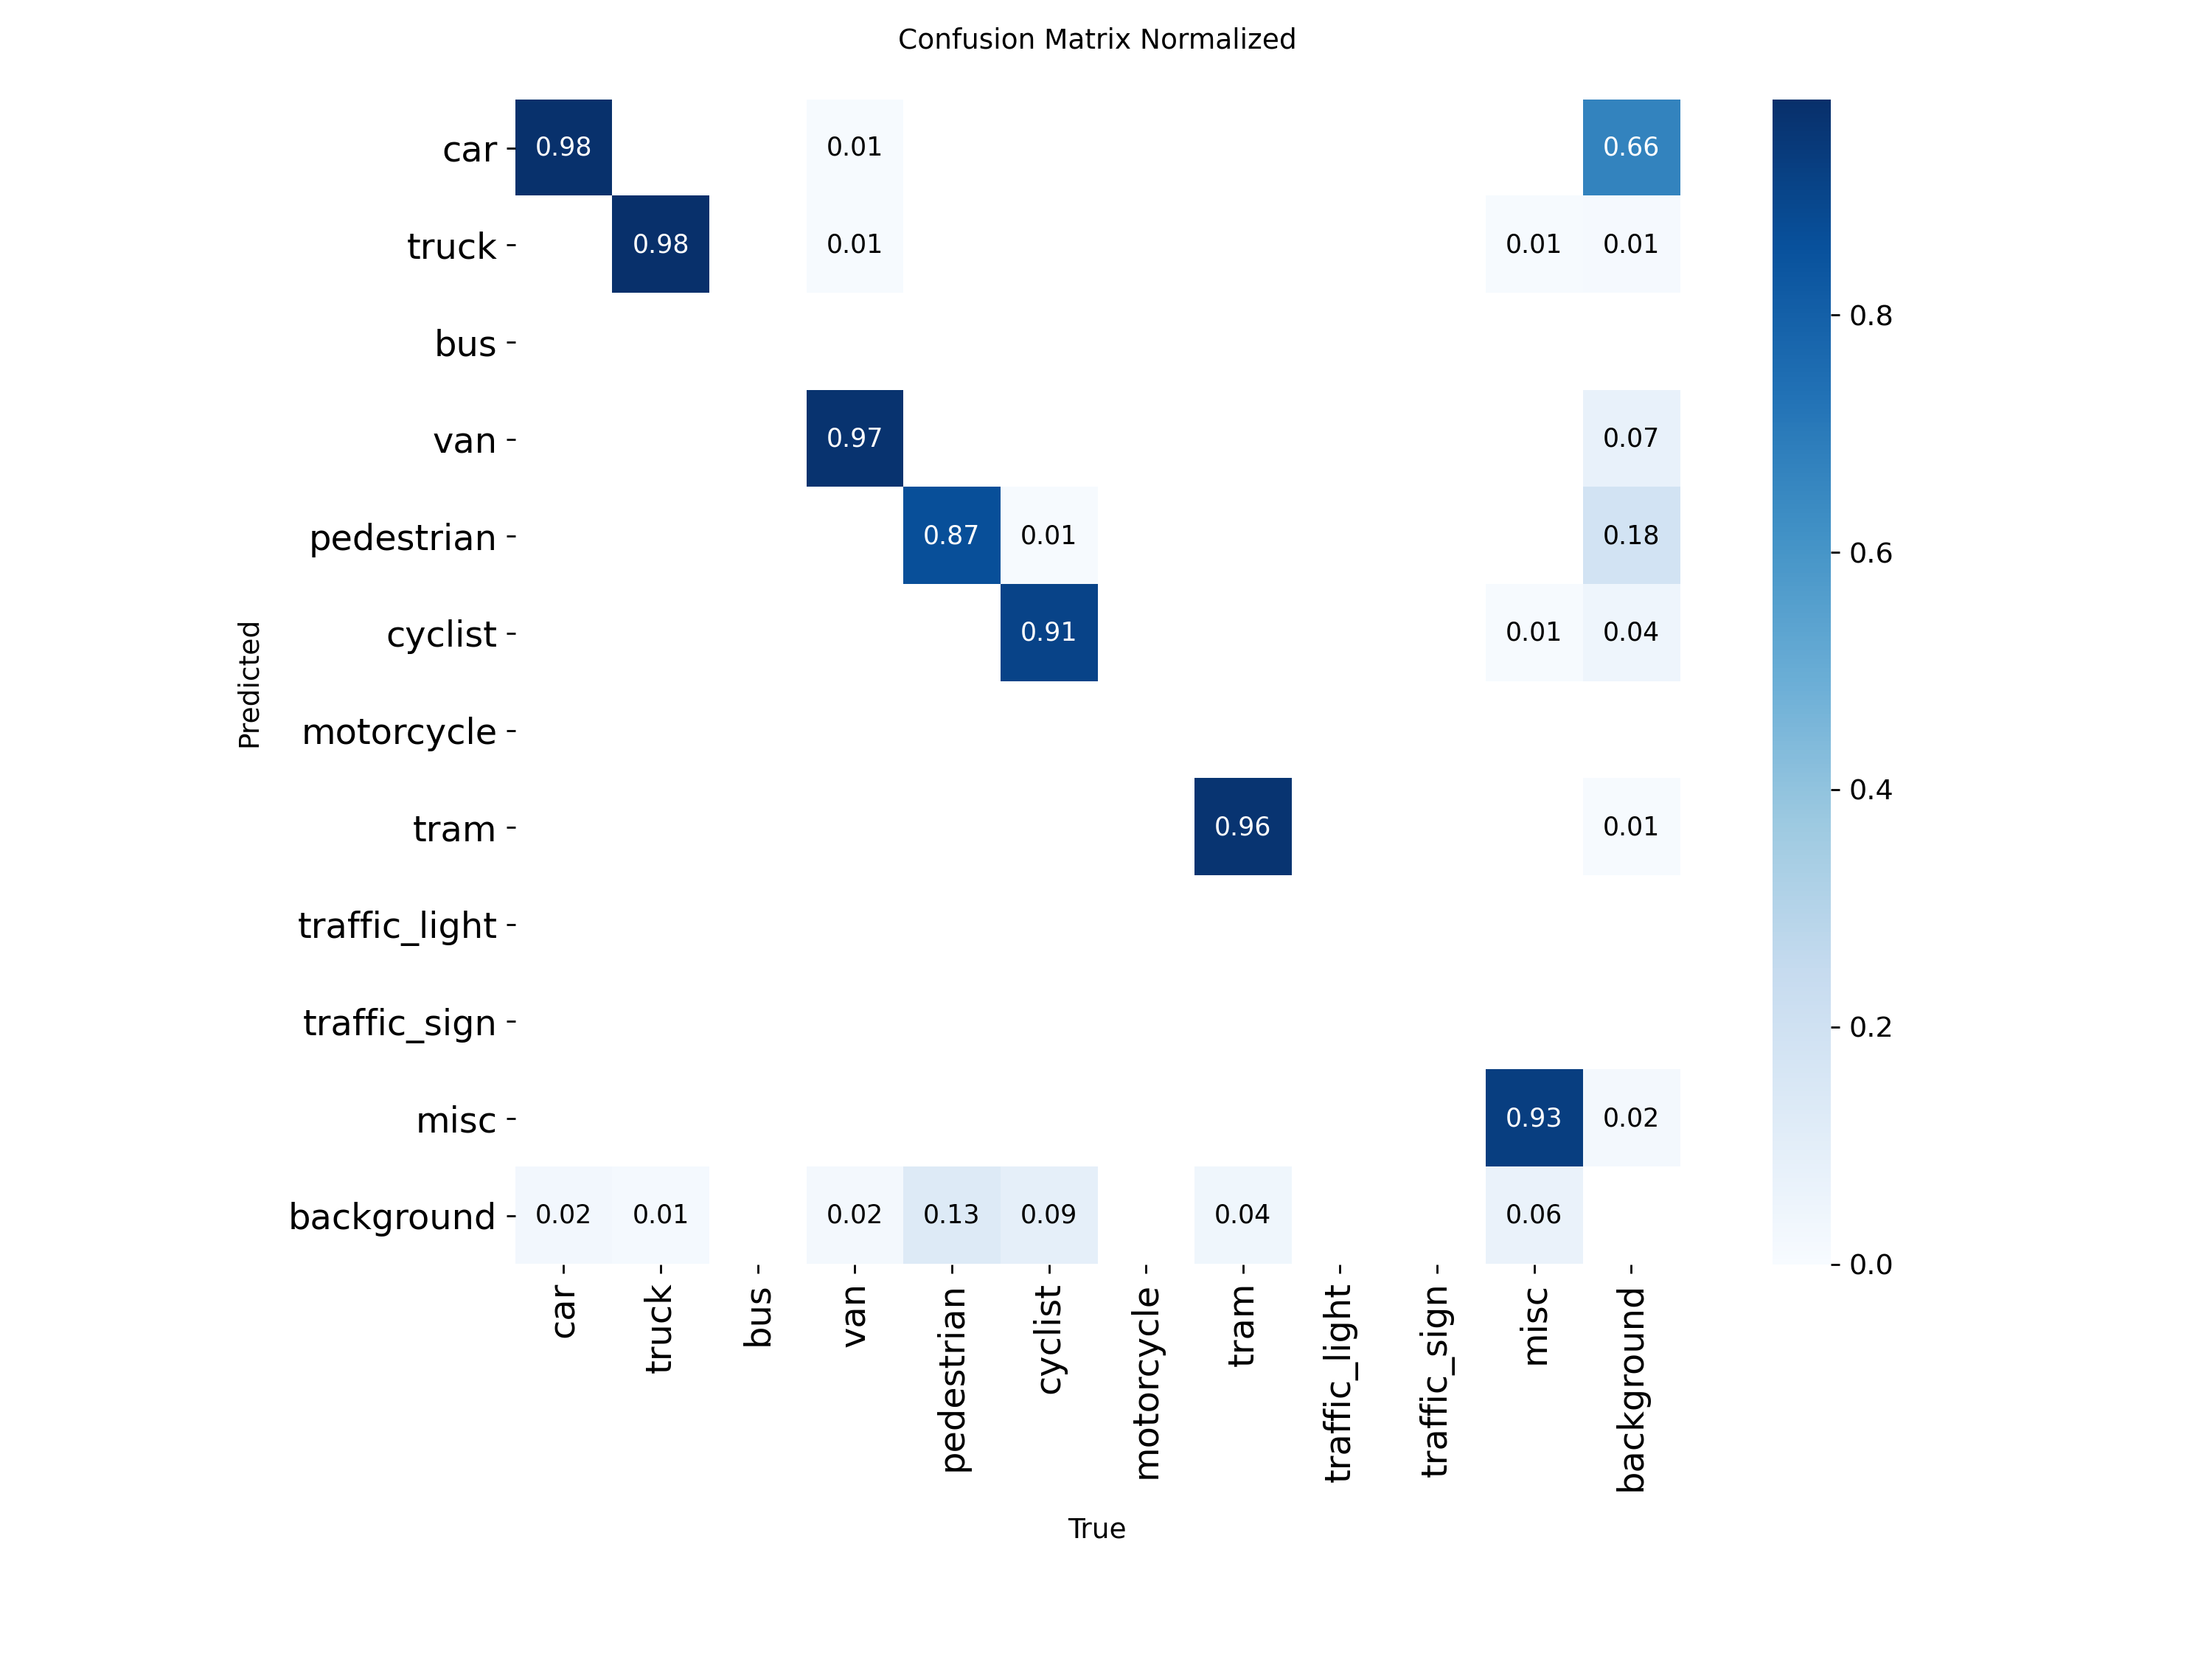
\includegraphics[width=0.92\columnwidth]{figures/confusion_matrix_normalized.png}
\caption{Normalised confusion matrix on the validation split. Diagonal entries
are correct classifications; off-diagonal entries show the categories most often
interchanged.}
\label{fig:confusion}
\end{figure}

\subsection{Effect of Training Schedule and Capacity}

Table~\ref{tab:progress} compares three configurations. Extending the medium
model from 50 to 500 epochs yields a larger improvement (\mbox{$+2.5$} points
mAP@0.5, \mbox{$+8.4$} points at the strict metric) than the subsequent increase
in capacity (\mbox{$+1.2$} and \mbox{$+2.2$} points). Under a constrained
accelerator budget, schedule length was the more productive expenditure.

\begin{table}[t]
\caption{Effect of training schedule and model capacity}
\label{tab:progress}
\centering
\footnotesize
\begin{tabular}{llrrr}
\toprule
Configuration & Model & Epochs & mAP@0.5 & mAP@0.5:0.95 \\
\midrule
Baseline & YOLO11m & 50  & 91.7 & 69.3 \\
Extended & YOLO11m & 500 & 94.2 & 77.7 \\
\textbf{Final} & \textbf{YOLO11x} & \textbf{300} & \textbf{95.4} & \textbf{79.9} \\
\bottomrule
\end{tabular}
\end{table}

\begin{figure}[t]
\centering
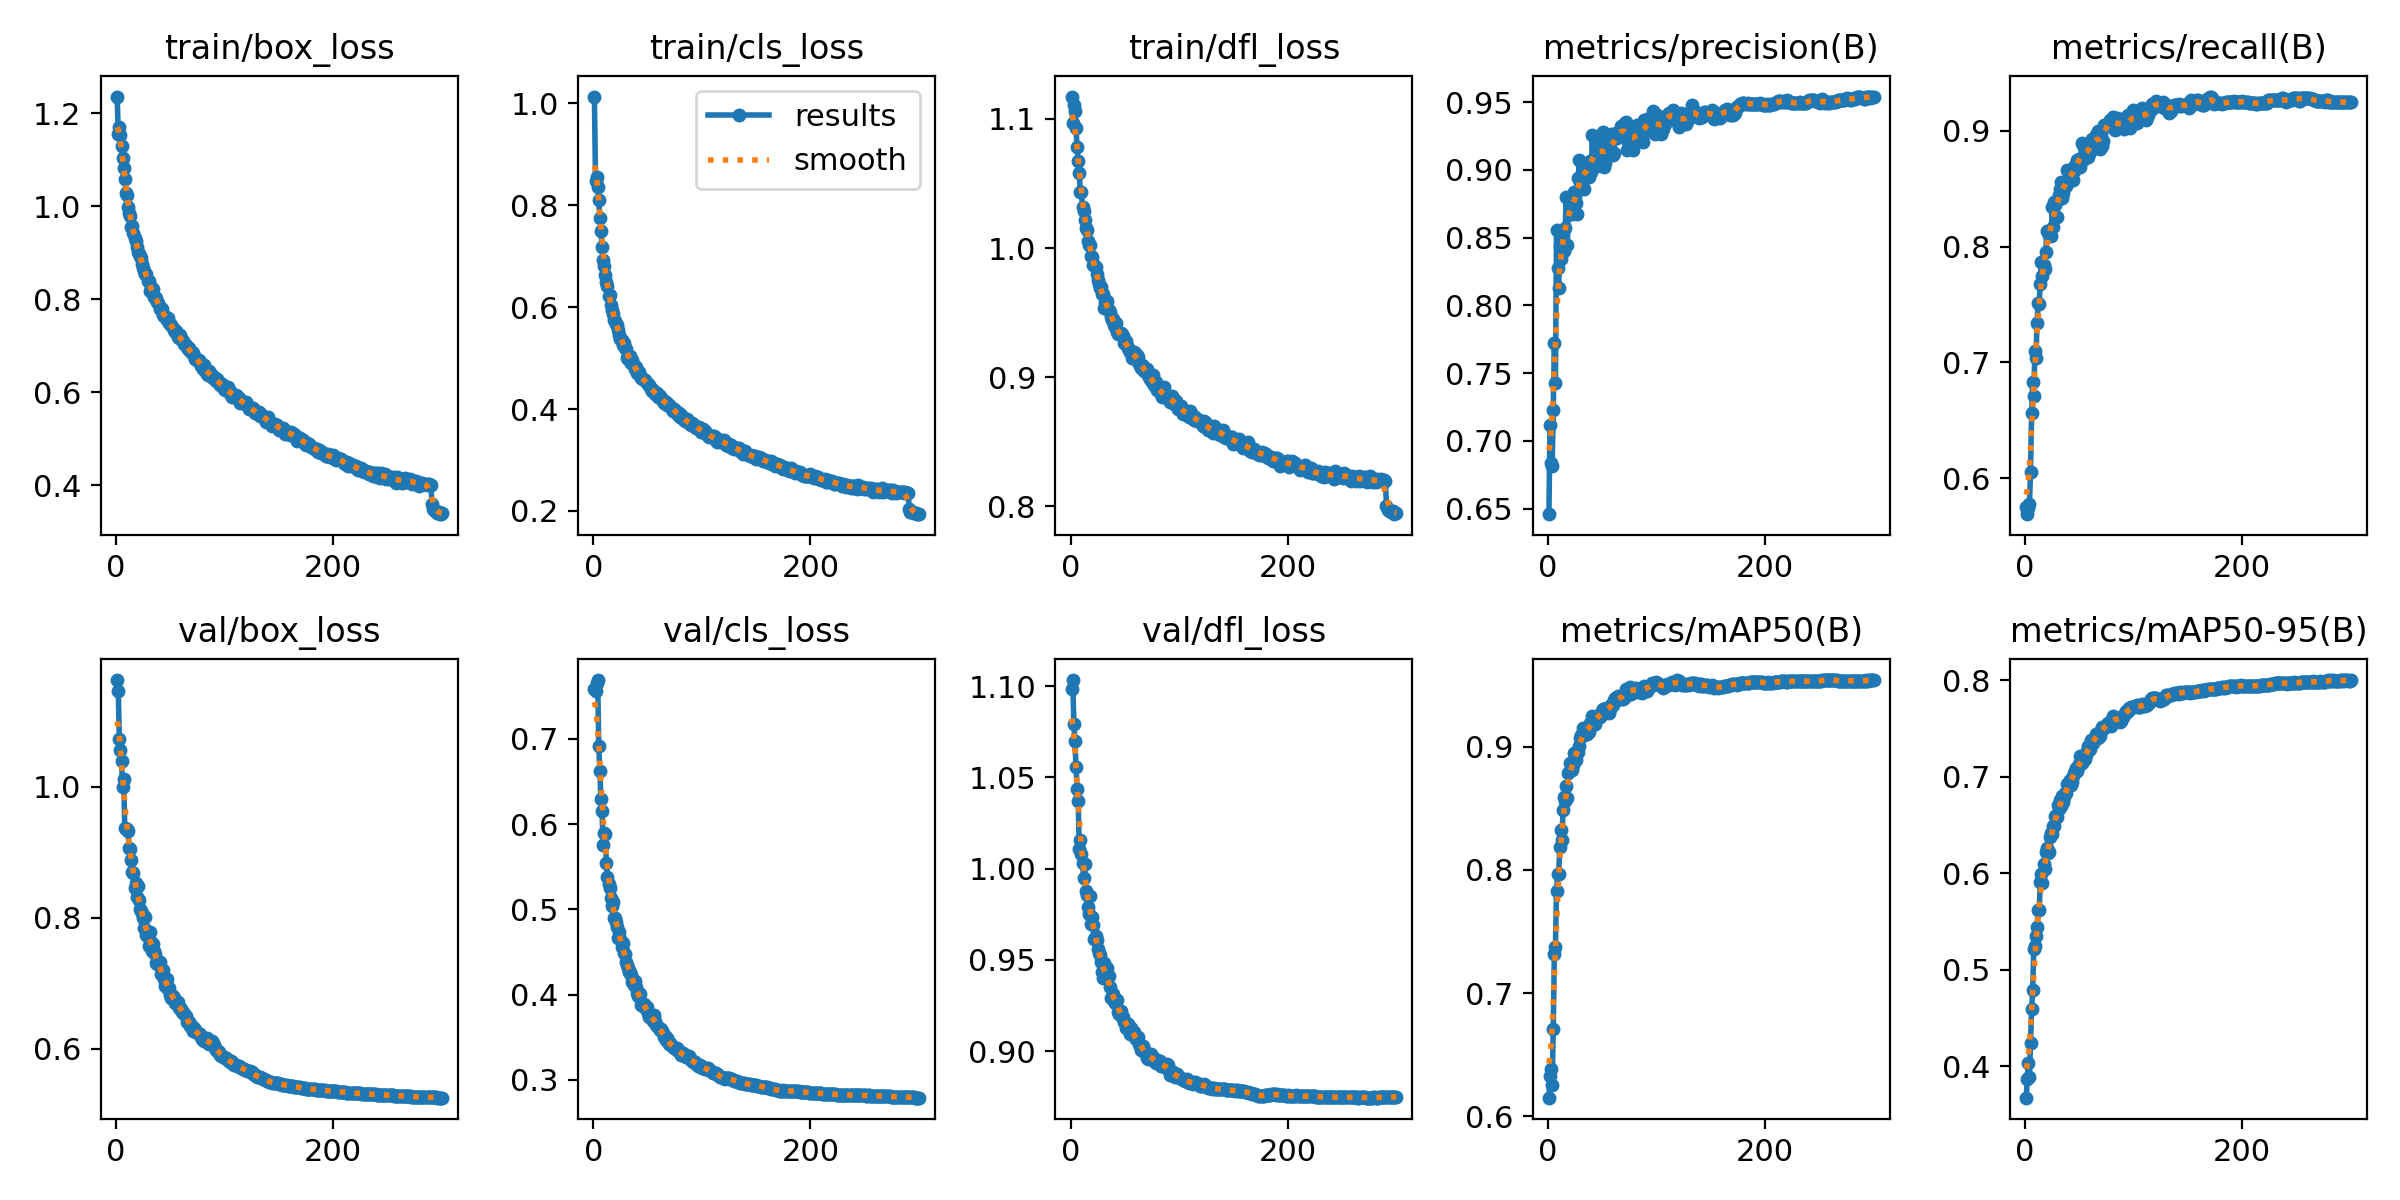
\includegraphics[width=\columnwidth]{figures/results.png}
\caption{Training behaviour of the final configuration. Box, classification and
distribution-focal losses converge without divergence on either split, and both
mAP measures rise monotonically before flattening.}
\label{fig:training}
\end{figure}

\subsection{End-to-End Pipeline}

Table~\ref{tab:pipeline} summarises a complete run over a 3{,}604-frame road
sequence. All six stages sustain 23.1\,frames per second at a mean latency of
43\,ms.

\begin{table}[t]
\caption{Complete pipeline over a 3{,}604-frame sequence}
\label{tab:pipeline}
\centering
\footnotesize
\begin{tabular}{lr}
\toprule
Measurement & Value \\
\midrule
Frames processed              & 3{,}604 \\
Throughput                    & 23.1 fps (43\,ms mean) \\
Collision alerts              & 69 (20 brake, 49 warning) \\
Frames with lane geometry     & 3{,}603 of 3{,}604 \\
Detections rejected by filter & 979 of 7{,}077 (13.8\,\%) \\
Detector parameters           & 56.8\,M (194.5 GFLOPs) \\
\bottomrule
\end{tabular}
\end{table}

An initial measurement of the same configuration returned 0.9\,frames per second.
The cause was placement of the depth model on the host processor rather than any
property of the pipeline; on the accelerator the identical code is approximately
twenty-five times faster. We record this because the two figures separate a
deployable system from an unusable one while differing in no respect other than
device placement---a diagnosis worth making before attributing latency to
architecture.

Fig.~\ref{fig:qualitative} shows representative output. Both alert tiers and the
tracking identifiers are drawn by the pipeline itself; no annotation was added
afterwards.

\begin{figure}[t]
\centering
\begin{minipage}{0.485\columnwidth}
  \centering
  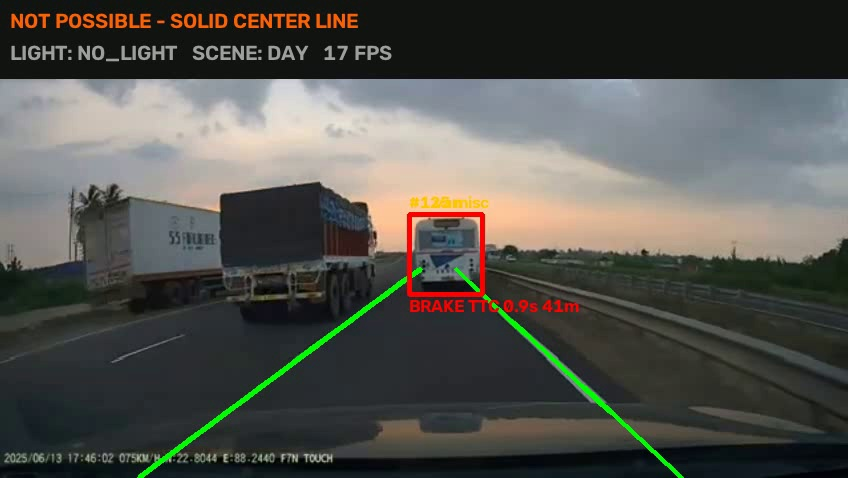
\includegraphics[width=\linewidth]{figures/BRAKE_01021.jpg}\\
  {\scriptsize (a) brake tier}
\end{minipage}\hfill
\begin{minipage}{0.485\columnwidth}
  \centering
  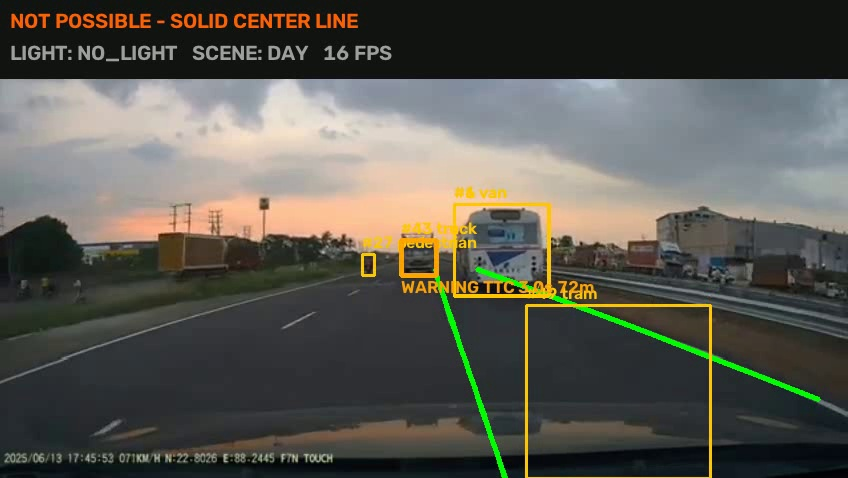
\includegraphics[width=\linewidth]{figures/WARNING_00423.jpg}\\
  {\scriptsize (b) warning tier}
\end{minipage}
\vspace{1.5mm}
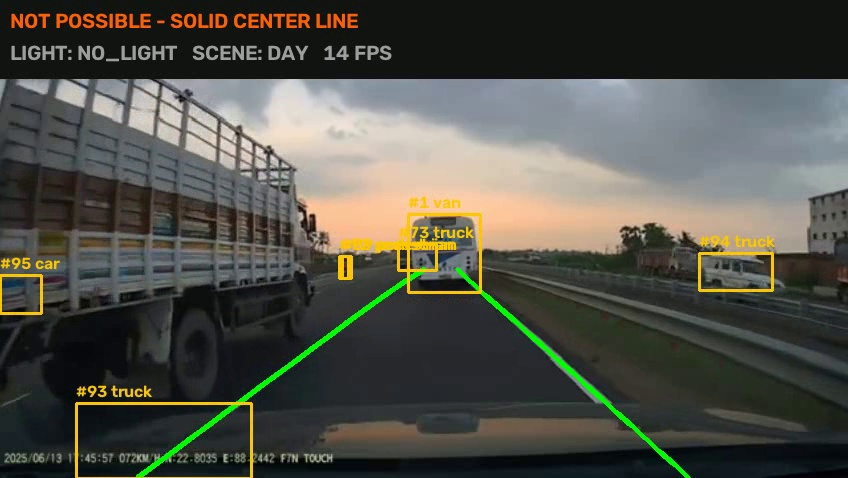
\includegraphics[width=0.92\columnwidth]{figures/BUSY_00682.jpg}\\
{\scriptsize (c) dense traffic, multiple simultaneous tracks}
\caption{Pipeline output. (a) and (b) show the two collision alert tiers with
distance and time-to-collision; (c) shows simultaneous tracking under dense
traffic.}
\label{fig:qualitative}
\end{figure}

\subsection{Plausibility Filter}

The filter removed 979 of 7{,}077 size-checked candidates. In an earlier
configuration using a narrower tolerance under an uncalibrated focal length, the
rejection rate reached approximately 27\,\% and included large numbers of vehicle
classes, indicating suppression of genuine objects rather than spurious ones.
Widening the tolerance in the uncalibrated regime, as described in
Section~\ref{sec:filter}, reduced the rate to 13.8\,\%. The episode illustrates
the intended asymmetry: an uncertain calibration should relax the admission
criterion, not tighten it.

%-----------------------------------------------------------------------------
%  TODO(authors): this subsection is written but its numbers are NOT yet
%  measured.  Run  training/pbs/india_step1_prepare.pbs  then
%  training/pbs/india_step2_compare.pbs, then replace every XX.X below with the
%  printed values and delete this comment together with the \textcolor markers.
%  DO NOT submit the paper with placeholder values still present.
%-----------------------------------------------------------------------------
\subsection{Adaptation to Unstructured Traffic}
\label{sec:india}

Sections~\ref{sec:limits} notes that the evaluated checkpoint is trained on
structured-road data only. To quantify what that costs on the target domain, and
what supervised adaptation recovers, we conduct a controlled comparison in which
a single held-out split of Indian traffic imagery \cite{iisc2025uvh26} serves as
the common test set for two models: the structured-road checkpoint evaluated
directly, and the same checkpoint after fine-tuning on the union of the original
corpus and the Indian training split. Because both are scored on identical data,
the difference is attributable to training distribution alone.

Fine-tuning proceeds from the existing checkpoint rather than from
general-purpose initialisation, on the reasoning that the backbone already
encodes road-scene structure and only the classification head must accommodate
the additional categories. Following the argument of \cite{kumar2025driveindia}
regarding sequential adaptation, the two corpora are merged and trained jointly
rather than in sequence, so that the original categories continue to receive
gradient signal. Table~\ref{tab:india} additionally reports the adapted model
re-evaluated on the original validation split, which tests whether that
precaution held.

\begin{table}[t]
\caption{Adaptation to unstructured traffic. Rows (A) and (B) are scored on an
identical held-out split of Indian traffic imagery; row (C) re-scores the
adapted model on the original structured-road split to test for forgetting.}
\label{tab:india}
\centering
\footnotesize
\begin{tabular}{llrr}
\toprule
 & Training data & mAP@0.5 & mAP@0.5:0.95 \\
\midrule
\multicolumn{4}{l}{\textit{Evaluated on the Indian test split}}\\
(A) & Structured-road only & XX.X & XX.X \\
(B) & \;\;$+$ Indian corpus (joint) & \textbf{XX.X} & \textbf{XX.X} \\
\midrule
\multicolumn{4}{l}{\textit{Evaluated on the original structured-road split}}\\
     & Before adaptation & 95.4 & 79.9 \\
(C) & After adaptation & XX.X & XX.X \\
\bottomrule
\end{tabular}
\end{table}

The gap between rows (A) and (B) measures the domain shift directly, in the same
manner as the adaptation experiments reported for this corpus by its authors
\cite{iisc2025uvh26}. Row (C) indicates whether joint training preserved
performance on the original distribution.

%=============================================================================
\section{Limitations}
\label{sec:limits}

We state the system's untrained capabilities explicitly, since each traces to a
data deficiency rather than an implementation defect and each therefore implies a
different remedy.

\textbf{Four declared classes carry no training examples.} The label space
defines traffic lights, traffic signs, buses and motorcycles, but the merge that
produced this checkpoint drew from a single structured-road source containing
none of them. Validation consequently reports seven classes rather than eleven.
No modification to the model can address this; a corpus containing the
categories is required.

% TODO(authors): once Section VI-E carries measured numbers, this paragraph
% should be reduced to the two corpora still unused, and the sentence about
% adaptation not having been performed must be deleted.
\textbf{Adaptation is demonstrated on one corpus only.} Section~\ref{sec:india}
quantifies adaptation using a single Indian corpus \cite{iisc2025uvh26}.
Conversion pipelines for two further corpora
\cite{varma2019idd, kumar2025driveindia} are implemented and tested but not yet
exercised, so the reported gain reflects one distribution rather than Indian
road conditions in general. The headline accuracy in
Table~\ref{tab:perclass} remains a structured-road measurement and should not be
read as performance on unstructured traffic.

\textbf{The overtaking verdict is conservative in the absence of marking type.}
Without a reliable solid-versus-broken classification the legality condition
cannot be satisfied, and the verdict remains \textit{not permitted}. This is the
intended fail-safe rather than a malfunction, but it does mean the module is
inactive on sequences lacking marking-type input.

\textbf{Monocular depth is less reliable than active ranging.} Distance and hence
time-to-collision inherit the error characteristics of learned monocular depth. A
system with an active range sensor would obtain more dependable distances; the
camera-only choice reflects a deployability constraint and should be recognised
as a trade-off.

%=============================================================================
\section{Conclusion and Future Work}

We have presented a monocular perception pipeline that integrates detection,
tracking, lane and corridor estimation, metric depth and two decision layers
within a single pass, attaining 95.4\,\% mAP@0.5 and sustaining 23.1\,frames per
second on an H100 accelerator. The system's distinguishing commitments are a
degradation contract exercised under real deployment failure, and the expression
of safety-relevant quantities in physical rather than image units.

Section~\ref{sec:india} establishes that supervised adaptation on a single
Indian corpus recovers a substantial part of the domain gap. Four directions
follow. Extending that adaptation to the two remaining corpora
\cite{varma2019idd, kumar2025driveindia}, for which the conversion
infrastructure is already complete, would test whether the gain generalises
beyond one distribution. Incorporating a source containing traffic lights and
signs would render four presently untrainable classes trainable. Camera
calibration would narrow the plausibility filter from its uncertainty-widened
interval and supply metric curvature. Finally, supervised training of the
drivable-corridor segmenter would replace the present classical-vision
substitute, improving lane estimation precisely where painted markings are
unavailable.

%=============================================================================
\begin{thebibliography}{00}

\bibitem{geiger2012kitti}
A.~Geiger, P.~Lenz, and R.~Urtasun, ``Are we ready for autonomous driving? The
KITTI vision benchmark suite,'' in \textit{Proc. IEEE Conf. Comput. Vis. Pattern
Recognit. (CVPR)}, Providence, RI, USA, Jun. 2012, pp.~3354--3361.

\bibitem{pan2018scnn}
X.~Pan, J.~Shi, P.~Luo, X.~Wang, and X.~Tang, ``Spatial as deep: Spatial CNN for
traffic scene understanding,'' in \textit{Proc. AAAI Conf. Artif. Intell.
(AAAI)}, New Orleans, LA, USA, Feb. 2018, pp.~7276--7283.

\bibitem{varma2019idd}
G.~Varma, A.~Subramanian, A.~Namboodiri, M.~Chandraker, and C.~V. Jawahar,
``IDD: A dataset for exploring problems of autonomous navigation in
unconstrained environments,'' in \textit{Proc. IEEE Winter Conf. Appl. Comput.
Vis. (WACV)}, Waikoloa Village, HI, USA, Jan. 2019, pp.~1743--1751.

\bibitem{kumar2025driveindia}
R.~Kumar, D.~S. Reddy, and P.~Rajalakshmi, ``DriveIndia: An object detection
dataset for diverse Indian traffic scenes,'' in \textit{Proc. IEEE Int. Conf.
Intell. Transp. Syst. (ITSC)}, 2025.

\bibitem{iisc2025uvh26}
Artificial Intelligence and Robotics Initiative (AIM), Indian Institute of
Science, ``The Urban Vision Hackathon dataset and models: Towards image
annotations and accurate vision models for Indian traffic,'' Tech. Rep.
UVH-26-v1.0, Indian Institute of Science, Bengaluru, India, Nov. 2025.

\bibitem{redmon2016yolo}
J.~Redmon, S.~Divvala, R.~Girshick, and A.~Farhadi, ``You only look once:
Unified, real-time object detection,'' in \textit{Proc. IEEE Conf. Comput. Vis.
Pattern Recognit. (CVPR)}, Las Vegas, NV, USA, Jun. 2016, pp.~779--788.

\bibitem{ultralytics2024yolo11}
G.~Jocher and J.~Qiu, ``Ultralytics YOLO11,'' software release, Ultralytics,
2024. [Online]. Available: \url{https://github.com/ultralytics/ultralytics}

\bibitem{zheng2022clrnet}
T.~Zheng, Y.~Huang, Y.~Liu, W.~Tang, Z.~Yang, D.~Cai, and X.~He, ``CLRNet: Cross
layer refinement network for lane detection,'' in \textit{Proc. IEEE/CVF Conf.
Comput. Vis. Pattern Recognit. (CVPR)}, New Orleans, LA, USA, Jun. 2022,
pp.~898--907.

\bibitem{qin2024ufldv2}
Z.~Qin, P.~Zhang, and X.~Li, ``Ultra fast deep lane detection with hybrid
anchor driven ordinal classification,'' \textit{IEEE Trans. Pattern Anal. Mach.
Intell.}, vol.~46, no.~5, pp.~2555--2568, May 2024.

\bibitem{zhang2022bytetrack}
Y.~Zhang, P.~Sun, Y.~Jiang, D.~Yu, F.~Weng, Z.~Yuan, P.~Luo, W.~Liu, and
X.~Wang, ``ByteTrack: Multi-object tracking by associating every detection
box,'' in \textit{Computer Vision -- ECCV 2022}, Lecture Notes in Computer
Science, vol.~13682. Cham, Switzerland: Springer, 2022, pp.~1--21.

\bibitem{yang2024depthv2}
L.~Yang, B.~Kang, Z.~Huang, Z.~Zhao, X.~Xu, J.~Feng, and H.~Zhao, ``Depth
Anything V2,'' in \textit{Advances in Neural Information Processing Systems
(NeurIPS)}, vol.~37, 2024.

\bibitem{li2021zerodce}
C.~Li, C.~Guo, and C.~C. Loy, ``Learning to enhance low-light image via
zero-reference deep curve estimation,'' \textit{IEEE Trans. Pattern Anal. Mach.
Intell.}, vol.~44, no.~8, pp.~4225--4238, Aug. 2022.

\bibitem{lian2022geoconsistency}
Q.~Lian, B.~Ye, R.~Xu, W.~Yao, and T.~Zhang, ``Exploring geometric consistency
for monocular 3D object detection,'' in \textit{Proc. IEEE/CVF Conf. Comput.
Vis. Pattern Recognit. (CVPR)}, New Orleans, LA, USA, Jun. 2022,
pp.~1685--1694.
%  Verified: openaccess.thecvf.com CVPR 2022 proceedings.

\bibitem{hartley2004multiple}
R.~Hartley and A.~Zisserman, \textit{Multiple View Geometry in Computer Vision},
2nd~ed. Cambridge, U.K.: Cambridge Univ. Press, 2004.

\end{thebibliography}

\end{document}
